%!TEX root = ../main.tex

\begin{frame}
    \frametitle{Starting Point}

    \begin{itemize}
        \item A collection of files on your computer (data, code, notes, ...)
        \item Changes to files and new files over time
        \item Interested in preserving the history 
        of these changes
        \item Want to be able to share work across users \& systems.
        \item Want to work on pieces in parallel without corrupting code.
    \end{itemize}
\end{frame}

\begin{frame}
    \frametitle{In one sentence...}
    ``Version Control is a system that records changes to a file or set of files
    over time so that you can recall specific versions later'' \citep{ChaconHamano2009}.
\end{frame}

\begin{frame}
    \frametitle{Version Control Evolving}
    \begin{itemize}
        \item Middle Ages - \href{http://en.wikipedia.org/wiki/Bible_translations}{Copying the Bible}
        \begin{itemize}
            \item Each version was handwritten
            \item Used margins for corrections
            \item Induced regional heterogeneity
        \end{itemize}
        \item The modern Bible scribe
        \begin{itemize}
            \item Copy/paste versions to an archive
            \item File name tags for different versions: \\ \url{mainFile_addingKrogerRobustness_fixedError_20130211.m}
            \item Include a readme
        \end{itemize}
        \item Post-modern methods of Version Control
        \begin{itemize}
            \item Version Control Systems
            \begin{itemize}
                \item Localized (\href{http://en.wikipedia.org/wiki/Revision_Control_System}{rcs})
                \item Centralized (CVS, \href{http://en.wikipedia.org/wiki/Apache_Subversion}{Subversion}, Perforce)
                \item Distributional (Git, Mercurial, Bazaar, Darcs)
            \end{itemize}
        \end{itemize}
    \end{itemize}
\end{frame}

%\begin{frame}[c]\frametitle{Concepts of Version Control Systems}
%    \begin{center}
%        \tikzstyle{concept}=[draw, rectangle, text centered, text width=2.5cm,
%        fill=black!20, rounded corners]
%        \tikzstyle{example}=[draw, rectangle, text centered, text width=3cm,
%        fill=black!10, rounded corners]
%        \tikzstyle{file}=[draw, rectangle, text centered, text width=1cm,
%        fill=black!5]        
%
%        \begin{tikzpicture}
%            \node [concept] (central) {Remote file system};
%            \node [concept, below of=central, node distance=3cm] (local) {Local file system};
%            \node [example, right of=central, node distance=4cm] (cex) {Github Server};
%            \node [example, right of=local, node distance=4cm] (lex) {Pam's Computer};
%            \node [file,below of=central,xshift=0.8cm] (a) {\small File A};
%            \node [file,below of=a] (b) {\small File B};
%
%            \draw [dotted, <->, thick] (central) -- (local);
%            \draw [dotted] (central) -- (cex);
%            \draw [dotted] (local) -- (lex);
%
%        \end{tikzpicture}        
%    \end{center}
%\end{frame}

\begin{frame}[c]\frametitle{Distributional Version Control Systems}
    \begin{itemize}
        \item Network of repository copies (mirrors)
        \item Identical, full copies of the data
        \item Remote storage in the cloud (github, bitbucket)
    \end{itemize}        
\end{frame}

\begin{frame}[c]\frametitle{DVCS Structure}
        \begin{figure}[h!]
            \label{fig_label}\vspace{0.2cm}
                \scalebox{0.35}{\includegraphics{figures/dvcs}}            
        \end{figure}
\end{frame}

\newgeometry{left=0cm,right=0cm,top=0.2cm}
\begin{frame}[fragile]\frametitle{\centerline{Version Control in Economic Research}}
    \begin{minipage}[b]{0.55\paperwidth}
        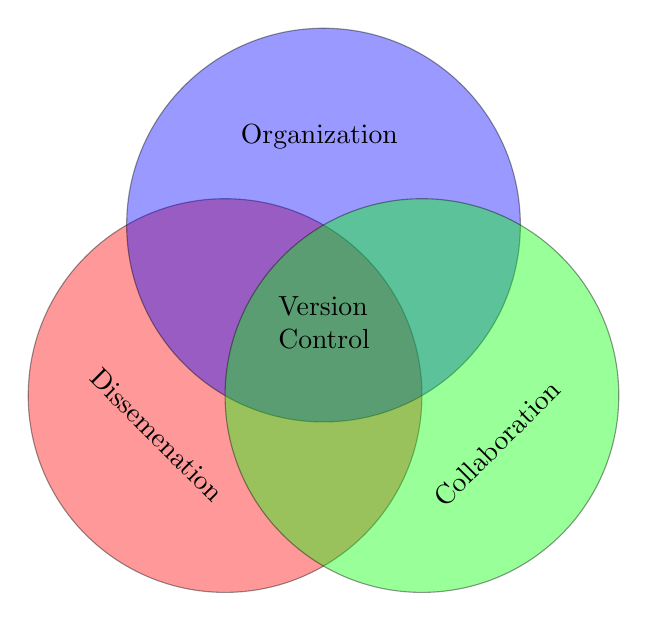
\begin{tikzpicture} \raggedright
          \tikzset{venn circle/.style={draw,circle,minimum width=5cm,fill=#1,opacity=0.4}}

          \node [venn circle = red] (left) at (0,0) {};
          \node [venn circle = blue] (top) at (60:2.5cm) {};
          \node [venn circle = green] (right) at (0:2.5cm) {};

          \node [rotate=-45] (lefttext) at (210:1cm) {Dissemenation};
          \node [rotate=45] (righttext) at (-10:3.5cm) {Collaboration};
          \node (toptext) at (70:3.5cm) {Organization};
          \node [text width=1.5cm](center) at (33:1.7cm) {Version Control};


        \end{tikzpicture}
    \end{minipage}
    \begin{minipage}[b]{0.4\paperwidth}
        \raggedleft
        \begin{itemize}
            \item Organization
                \begin{itemize}
                    \item Contemporaneity
                    %seamless updating
                    \item Workflow
                    %branching, milestones
                    \item Project Management
                    \item Progress tracking
                    \item Security
                    %backup, access
                \end{itemize}
            \item Dissemenation
                \begin{itemize}
                    \item Availability
                    \item Reproducibility
                    \item Transparency
                    \item Extendability
                \end{itemize}
             \item Collaboration
                \begin{itemize}
                    \item Visibility
                    %oversight, logging, responsibility, part and the whole
                    \item Communication
                    %issue creation, conflict resolution, foresight
                    \item Coordination
                \end{itemize}
        \end{itemize}
    \end{minipage}
\end{frame}
\restoregeometry

\begin{frame}\frametitle{Organization}
    \begin{itemize}
        \item Always stay up-to-date, always have a backup
        \item Explore alternative workflows--diverge and converge
        \item Branching Workflow--\href{http://git-scm.com/book/en/Git-Branching}{at ease with experimentation}
        \item Quickly compare and merge versions 
        \item Retain an (annotated) \href{http://git-scm.com/book/en/Git-Basics-Viewing-the-Commit-History}{historical record} of your work
        \item Manage \href{http://git-scm.com/book/en/Git-Internals-Transfer-Protocols}{access rights}
    \end{itemize}
\end{frame}


\begin{frame}
    \frametitle{Dissemenation}
    \begin{itemize}
        \item Self-contained source code
        \item Online visualization and availability
        \item Seamless integration with existing knowledge...
        \begin{itemize}
            \item Reduces burden to reproduce work
            \item Provides immediate stepping stone for future work
            \item Meaning more scientific progress!
        \end{itemize}
        \item Facilitates review of scientific work
        \begin{itemize}
            \item Too often overlooked and under-emphasized
        \end{itemize}
    \end{itemize}
    You'll believe me if you go on \href{https://github.com/}{Github.com}.
\end{frame}


\begin{frame}\frametitle{Collaboration}
    \begin{itemize}
        \item Increase oversight over project contributors
        \begin{itemize}
            \item Check logs for progress updates
            \item Set milestones and tag important project
            states
        \end{itemize}
        \item Quickly point-out issues (bugs)
        \item Resolve file conflicts
        \item Increase foresight
        \item At-ease with the newbies
        \begin{itemize}
            \item Erase mistakes
        \end{itemize}
        \item Non-linear project workflows
        \item Easily merge work from others
    \end{itemize}
\end{frame}

\begin{frame}[c]
    \begin{center}
        \Large Git
    \end{center}
\end{frame}